\documentclass{article}
\usepackage{amsmath}

% Placeholder paragraphs with text
\usepackage{blindtext}

% figures
\usepackage{graphicx}
\usepackage{float}

% No indent for new paragraphs
\setlength\parindent{0pt}



\begin{document}

\section{This is the highest level section header: some text}
\blindtext[1]

\subsection{This is a subsection: equations}
 
A simple equation:
\begin{equation}
x^2 + y^2 = 1
\end{equation}


% No indent for a single paragraph 
%\noindent
Multiple equations:
\begin{gather}
	x = 1 \\
	y = -1
\end{gather}

Aligned system of equations:
\begin{align}
\frac{\partial y}{\partial x} &= y ^ {\prime} (x) \\
\sum\limits_{i=1}^{N}y_i &= e^{\alpha + \beta x}
\end{align}

A new system to be aligned
\begin{align}
x ^ 2 + y ^ 2 &= 1 \\
a \& b &\& c \& d = \omega
\end{align}

\subsubsection{Subsubsection is here: a figure}
Figure:


\blindtext[2]


\begin{figure}[H]
\caption{This is figure title}
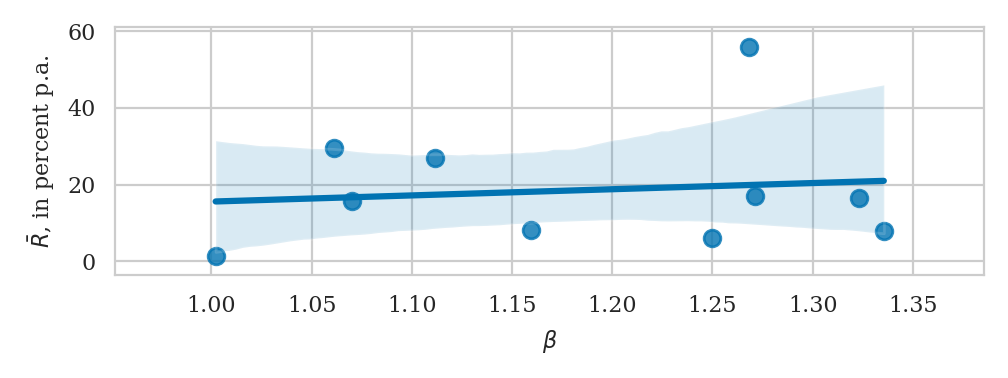
\includegraphics{../../figures/beta-vs-mu.png}
\end{figure}

\blindtext[1]

\begin{figure}[H]
\caption{This is figure title}
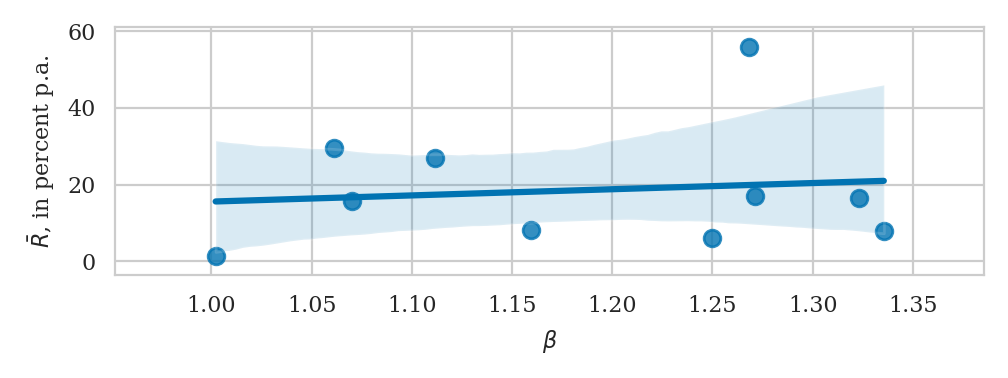
\includegraphics{../../figures/beta-vs-mu.png}
\end{figure}


\end{document}
